\documentclass[icelandic]{beamer}
\usepackage{amsmath,amssymb,latexsym,graphics}
\usepackage[english,icelandic]{babel}
\usepackage[utf8]{inputenc}
\usepackage{t1enc}
\usepackage{etoolbox}
\usepackage{tcolorbox}
\usepackage{pictex}
\usepackage{wrapfig}
\usepackage{pgf,tikz,pgfplots}
\pgfplotsset{compat=newest}
\usepackage{tkz-euclide}
\usepackage{tikz-cd}
\beamertemplatenavigationsymbolsempty
\setbeamertemplate{footline}[frame number]
\definecolor{von}{RGB}{235, 113, 37}
\setbeamercolor{block title}{fg=von}

%\input{preample}

%%%%%%%%%%%%%%%%%%%%%
%%%%% VARIABLES %%%%%

% Aspect ratio. Default 4:3, but 16:9 if WIDE is true.
\providetoggle{WIDE}
\settoggle{WIDE}{false}
\def\NAME{name}
\def\TITLE{title}
\def\FACULTY{faculty}
\def\SEMINAR{seminar}
\def\EMAIL{name@hi.is}

%%%%%%%%%%%%%%%%%%%%%%

\iftoggle{WIDE}{
    \usepackage[orientation=landscape,size=custom,width=16,height=9,scale=0.5,debug]{beamerposter} 
}{}

\title{\textbf{\large \TITLE}\\
    {\small \textbf{\NAME { }<\EMAIL>}}\\\vspace{-0.2cm}
{\scriptsize \FACULTY}\\
{\small \SEMINAR}\\\vspace{-0.2cm}
{\scriptsize \today}
}
\date{}
\usetheme{default}
\definecolor{haskolablatt}{RGB}{16,9,159}
\setbeamertemplate{frametitle}{
} 
\setbeamerfont{institute}{size=\scriptsize,series=\mdseries,parent=structure}
\setbeamerfont{date}{size=\scriptsize,series=\mdseries,parent=structure}
\setbeamersize{text margin left=.5cm}
\setbeamersize{text margin right=.5cm}
\setbeamercolor{title}{fg=haskolablatt,bg=white}
\setbeamercolor{author}{fg=haskolablatt}
\setbeamercolor{date}{fg=haskolablatt}
\setbeamercolor{item}{fg=haskolablatt}
\setbeamercolor{block title}{fg=haskolablatt}

\begin{document}
\iftoggle{WIDE}{
    \usebackgroundtemplate{\includegraphics[width=\paperwidth]{front169.png}}
% If you put background images in e.g. ~/Templates you can use the following:
 %   \usebackgroundtemplate{\includegraphics[width=\paperwidth]{\string~/Templates/front169.png}}
}{
    \usebackgroundtemplate{\includegraphics[width=\paperwidth]{front43.png}}
%    \usebackgroundtemplate{\includegraphics[width=\paperwidth]{\string~/Templates/front43.png}}
}


\begin{frame}
    \vspace{3cm}
    \pgfsetfillopacity{0.78}
\titlepage
\thispagestyle{empty}
\end{frame}

\usebackgroundtemplate{
\includegraphics[width=\paperwidth]{background.png}}
%\usebackgroundtemplate{
\includegraphics[width=\paperwidth]{\string~/Templates/background.png}}

\begin{frame}
    \begin{block}{Block}
        Asdf
        \pause
\begin{columns}[T] % align columns
\begin{column}{.48\textwidth}
Left columnt
\end{column}%
\hfill%
\begin{column}{.48\textwidth}
Right column
\end{column}
\end{columns}
    \end{block}
\end{frame}
\end{document}
